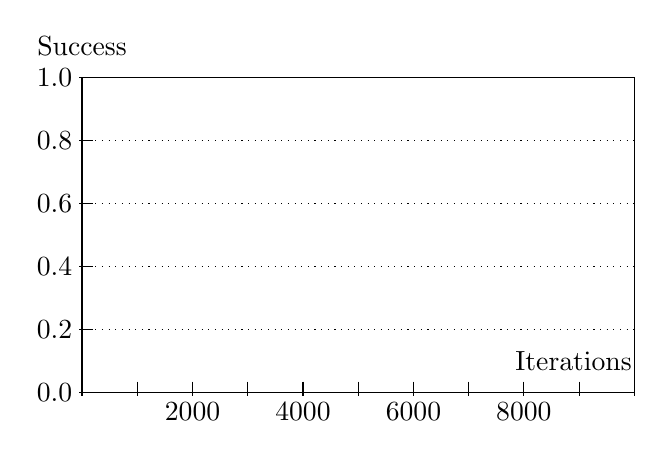
\begin{tikzpicture}[x=0.0007cm,y=4cm]
    % Draw the axes and grid lines
    \draw[-] (0,0) -- (0,1) -- (10000,1) -- (10000,0) -- cycle; 
    \draw[-,thin, dotted, ystep=0.2, xstep=10000] (0,0) grid (10000,1);
    \foreach \x in {0,1000,...,10000}  \draw [-,xshift=0](\x,4pt) -- (\x,-1pt);
    \foreach \y in {0.0,0.2,0.4,0.6,0.8,1.0}  \draw [-,yshift=0](4pt,\y) -- (-1pt,\y);
    \foreach \x/\xtext in {2000/2000, 4000/4000, 6000/6000, 8000/8000} \node at (\x,0) [below] {$\xtext$};
    \foreach \y/\ytext in {0.0,0.2,0.4,0.6,0.8,1.0}  \node at (0,\y) [left] {$\ytext$};
    \node at (0,1.1) {Success};
    \node at (8900,0.1) {Iterations};
    \draw[-] plot[mark=square,mark size=2,mark options={color=black}] 
			file {data/testMultiSolutionsR.CC.tikzdata};
    \draw[-,thin,densely dashed,gray] plot[mark=triangle,gray,mark size=3,mark options={color=gray}] 
			file {data/testMultiSolutionsR.CP.tikzdata};
    \draw[-] plot[mark=diamond,mark size=3,mark options={color=black}] 
			file {data/testMultiSolutionsR.SC.tikzdata};
    \draw[-,thin,densely dashed,gray] plot[mark=o,gray,mark size=2,mark options={color=gray}] 
			file {data/testMultiSolutionsR.SP.tikzdata};

\end{tikzpicture}
